% This file allows to produce either a separate PDF/PNG image
% See standalone documentation to understand underlying magic

\documentclass[tikz,convert={density=150,size=600,outext=.png}]{standalone}
\usetikzlibrary{shapes, calc, arrows, fit, positioning, decorations, patterns, decorations.pathreplacing, chains, snakes}
\input{../setup-web-fonts}
\input{../setup-packages}
\graphicspath{{../pictures/}} % path to pictures, trailing slash is mandatory.

% The actual drawing follows
\begin{document}
\begin{tikzpicture}[>=latex, font=\small]
    \node[] (gui) {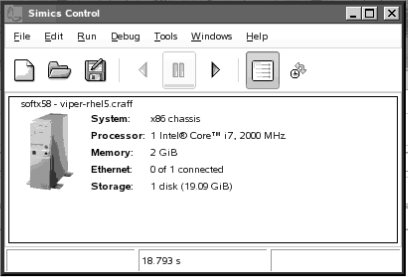
\includegraphics[width=2cm]{./gui.png}};
    \node[above=0.1cm of gui] {Графический интерфейс};
    
    \node[right = 1cm of gui]     (device1) {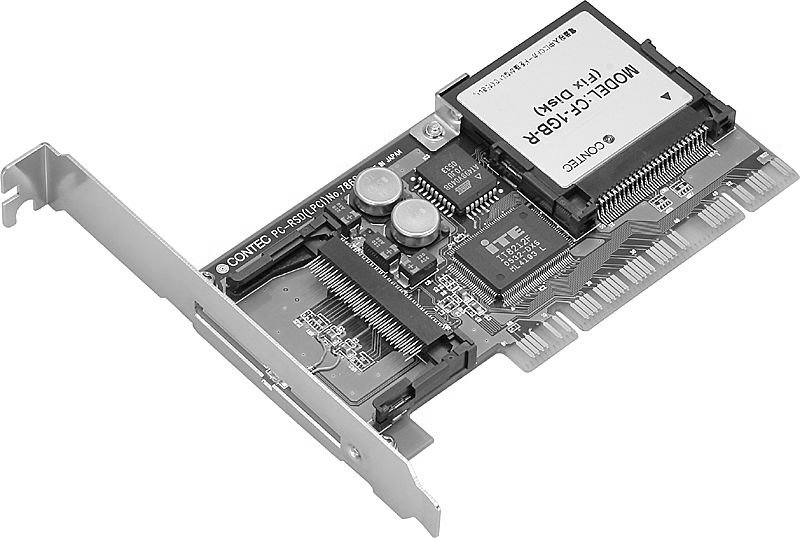
\includegraphics[height=1.5cm]{./device1.png}};
    \node[right = 0.2cm of device1] (device2) {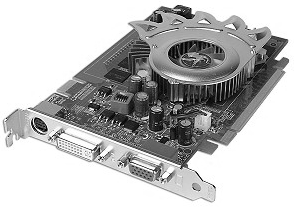
\includegraphics[height=1.5cm]{./device2.png}};
    \node[right = 0.2cm of device2] (device3) {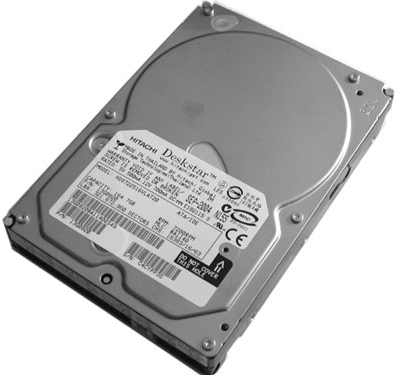
\includegraphics[height=1.5cm]{./device3.png}};
    
    \node[draw, inner sep= 2pt, fit=(device1) (device3)] (frame) {};
    
    \node[below = 2.5cm of gui] (cli) {
\includegraphics[height=1.5cm]{./cli.png}};
    
    \node[draw, circle, below = 0.7cm of device1] (core) {Ядро};
    
    \node[right = 3cm of cli] (python) {
\includegraphics[height=1.5cm]{./python.png}};
    \node[right = 0.2cm of python] (perl) {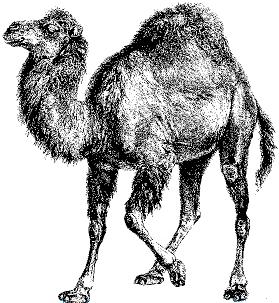
\includegraphics[height=1.5cm]{./perl.png}};
    \node[right = 0.2cm of perl] (lua) {
\includegraphics[height=1.5cm]{./lua.png}};
    
    \node[above=0.1cm of cli] {Командная строка};
    \node[above=0.1cm of perl] {Язык сценариев};
    \node[above=0.1cm of device2] {Модели устройств};
    
    \draw[<->, shorten >=0.8cm] (core) -- (gui);
    \draw[<->, shorten >=0.2cm] (core) -- (frame);
    \draw[<->, shorten >=0.8cm] (core) -- (cli);
    \draw[<->, shorten >=0.8cm] (core) -- (perl);
\end{tikzpicture}


\end{document}
